%%%%%%%%% ICML 2018 EXAMPLE LATEX SUBMISSION FILE %%%%%%%%%%%%%%%%%
%
%\documentclass{article}
%
%% Recommended, but optional, packages for figures and better typesetting:
%\usepackage{microtype}
%\usepackage{graphicx}
%
%\usepackage{subfig}
%\usepackage{color}
%
%% hyperref makes hyperlinks in the resulting PDF.
%% If your build breaks (sometimes temporarily if a hyperlink spans a page)
%% please comment out the following usepackage line and replace
%% \usepackage{icml2018} with \usepackage[nohyperref]{icml2018} above.
%\usepackage{hyperref}
%
%% Attempt to make hyperref and algorithmic work together better:
%\newcommand{\theHalgorithm}{\arabic{algorithm}}
%
%% Use the following line for the initial blind version submitted for review:
%\usepackage{sty_bst/icml}
%\usepackage{booktabs} % for professional tables
%\usepackage{amsmath}
%\usepackage{amssymb}
%\usepackage{multirow}
%\usepackage{xspace}
%
%
%% hyperref makes hyperlinks in the resulting PDF.
%% If your build breaks (sometimes temporarily if a hyperlink spans a page)
%% please comment out the following usepackage line and replace
%% \usepackage{icml2018} with \usepackage[nohyperref]{icml2018} above.
%\usepackage{hyperref}
%
%\newcommand{\todo}[1]{\textcolor{red}{#1}}
%\newcommand{\dd}[1]{\textcolor{blue}{#1}}
%\newcommand{\stopforward}{\textrm{sf}}
%\newcommand{\stopgradient}{\textrm{sg}}
%\newcommand{\petridishhard}{Isolated\xspace}
%\newcommand{\petridishsoft}{Joint\xspace}
%\newcommand{\Petridish}{Petridish\xspace}
%\newcommand{\PetridishCP}{Petridish-CP\xspace}
%\newcommand{\PetridishWS}{Petridish-WS\xspace}
%
%
%% The \icmltitle you define below is probably too long as a header.
%% Therefore, a short form for the running title is supplied here:
%%\icmltitlerunning{Submission and Formatting Instructions for ICML 2018}
%
%\begin{document}
%
%\twocolumn[
%\icmltitle{Guided Network Growth for Neural Architecture Search}
%
%% It is OKAY to include author information, even for blind
%% submissions: the style file will automatically remove it for you
%% unless you've provided the [accepted] option to the icml2018
%% package.
%
%% List of affiliations: The first argument should be a (short)
%% identifier you will use later to specify author affiliations
%% Academic affiliations should list Department, University, City, Region, Country
%% Industry affiliations should list Company, City, Region, Country
%
%% You can specify symbols, otherwise they are numbered in order.
%% Ideally, you should not use this facility. Affiliations will be numbered
%% in order of appearance and this is the preferred way.
%\icmlsetsymbol{equal}{*}
%
%\begin{icmlauthorlist}
%\icmlauthor{Aeiau Zzzz}{equal,to}
%\icmlauthor{Bauiu C.~Yyyy}{equal,to,goo}
%\icmlauthor{Cieua Vvvvv}{goo}
%\icmlauthor{Iaesut Saoeu}{ed}
%\icmlauthor{Fiuea Rrrr}{to}
%\icmlauthor{Tateu H.~Yasehe}{ed,to,goo}
%\icmlauthor{Aaoeu Iasoh}{goo}
%\icmlauthor{Buiui Eueu}{ed}
%\icmlauthor{Aeuia Zzzz}{ed}
%\icmlauthor{Bieea C.~Yyyy}{to,goo}
%\icmlauthor{Teoau Xxxx}{ed}
%\icmlauthor{Eee Pppp}{ed}
%\end{icmlauthorlist}
%
%\icmlaffiliation{to}{Department of Computation, University of Torontoland, Torontoland, Canada}
%\icmlaffiliation{goo}{Googol ShallowMind, New London, Michigan, USA}
%\icmlaffiliation{ed}{School of Computation, University of Edenborrow, Edenborrow, United Kingdom}
%
%\icmlcorrespondingauthor{Cieua Vvvvv}{c.vvvvv@googol.com}
%\icmlcorrespondingauthor{Eee Pppp}{ep@eden.co.uk}
%
%% You may provide any keywords that you
%% find helpful for describing your paper; these are used to populate
%% the "keywords" metadata in the PDF but will not be shown in the document
%\icmlkeywords{Machine Learning, ICML}
%
%\vskip 0.3in
%]
%
%% this must go after the closing bracket ] following \twocolumn[ ...
%
%% This command actually creates the footnote in the first column
%% listing the affiliations and the copyright notice.
%% The command takes one argument, which is text to display at the start of the footnote.
%% The \icmlEqualContribution command is standard text for equal contribution.
%% Remove it (just {}) if you do not need this facility.
%
%%\printAffiliationsAndNotice{}  % leave blank if no need to mention equal contribution
%\printAffiliationsAndNotice{\icmlEqualContribution} % otherwise use the standard text.
%
%\begin{abstract}
%When developing predictors for machine learning applications, practitioners often want to have simple and working predictors early and continue to improve them with available computational resources. 
%In this work, we propose a neural architecture search (NAS) algorithm that iteratively augments existing networks by adding shortcut connections and layers. At each iteration, we greedily select among the most cost-efficient models a parent model, and insert into it a number of candidate layers.  To learn which combination of additional layers to keep,  we simultaneously train their parameters and select the most promising candidates via feature selection techniques. The selected candidates are then jointly trained with the parent model.  Within 15 GPU-days, the proposed network growth NAS algorithm (\Petridish) can already find a model on CIFAR-10 that achieves 2.79\% error rate using 2.8M parameters.  We also transfer the model to ILSVRC2012, and it achieves 25.4\% top-1 error rate using 6.2M parameters and 810M multiply-adds. 
%Furthermore, unlike recent studies of NAS that almost exclusively focus on the small search space of repeatable network modules (cells), this work also shows that a direct search among the more general networks (macro) can also find cost-effective models when macro search is allowed to start with the same initial models as cell search does. 
%\end{abstract}

\section{Introduction}
\label{sec:nas_introduction}

Deep neural networks have achieved state-of-the-art performance on many large scale supervised learning tasks across many domains like computer vision, natural language processing and audio and speech-related tasks. But most gains have come from manually designed architectures which have inspired further improvements via careful experimentation coupled with significant experience and intuition of a skilled practitioner. Such skilled practitioners usually have significant domain knowledge of the task at hand that allows them to make rapid progress. But the fact remains that the task of designing a deep network architecture from scratch remains mostly a game of trial and error. As a consequence there has been significant effort in the community to address this issue via attempts to design algorithms that automatically find good architectures and informally referred to as AutoDNN and/or Neural Architecture Search (NAS) \cite{nas}. 

NAS literature can be broadly categorized along three main dimensions: 1. search space 2. search procedure and 3. performance estimation strategy during the search procedure. The search space can be broadly further divided to methods that search either 1. a more general space of architectures often termed as macro-search or 2. a more constrained search space called micro or cell-search. In cell-search a good outer skeleton is often assumed. For example in image classification datasets it is common to often assume either ResNet~\citep{resnet} or DenseNet~\cite{densenet} style outer skeletons. The search can then be restricted to finding cells that fill in the slots in the outer skeleton so that the overall architecture has good performance. Cell-search is much more popular due to a number of reasons: 1. One can leverage domain knowledge of experts who have painstakingly come up with good architectures and focus the search to a smaller space. 2. Transfer to larger datasets where more capacity is often needed can be obtained by trivially stacking many cells to create larger networks. The very aspects that make cell-search attractive also prevent it from providing a truly general solution: when good outer skeletons are not available for novel domains/datasets or there is reason to believe that significant performance is left on the table, cell-search cannot be applied. By restricting the search space it is quite possible that significant performance is left on the table. On large datasets in production environments this feature is especially important. Macro-search in principle doesn't suffer from any of the above limitations but suffers from searching a much more general and larger architecture space. 

In this work we propose a method for growing networks from small to large where we opportunistically add layers inspired by the ``cascade correlation'' work of \cite{cascadecorr}. We term our approach \Petridish. \Petridish can be used with both macro and cell-search spaces. Importantly \Petridish achieves better performance on macro search spaces than any other NAS algorithm which considers macro search results. Furthermore the final results achieved by \Petridish macro are comparable to those of the current best cell-search methods including that of \Petridish cell-search methods.

\begin{itemize}
\item We propose an approach to increase complexity of neural networks during training iteratively. We alternate between two phases. The first expands the model with potential shortcut connections and train them jointly. The second phase trim the previous potential connections using feature selection and continue training the model. 
\item The proposed approach can be applied to both improve a small repeatable pattern, called cell, and improve the macro network architecture directly, unlike most popular approaches that only focus on cells. This opens up neural architecture search to fields where no domain knowledge of the macro structure exists. 
\item On cell-search, the proposed method finds a model that achieves 2.61\% error rate on CIFAR10 using 2.9M parameters within 5 GPU-days. 
%The model achieves \% error rate on ILSVRC2012 using M parameters and M multi-adds.
\item On macro-search, the proposed method finds a model that achieves 2.83\% error rate on CIFAR10 using 2.2M parameters within 5 GPU-days. 
%The model achieves \% error rate on ILSVRC2012 using M parameters and M multi-adds.
\item The proposed approach can warm start from existing networks, leveraging previous training results. Furthermore, it directly expands models on the lower convex hull of error rate vs. flops and is hence able to naturally produce a gallery of cost-effective models which is critical for production serving needs. 
\end{itemize}


\section{Background and References}
\label{sec:nas_background}
%\begin{itemize}
%    \item Cascade-correlation
%    \item NAS. (RL. EA. Gradient based.) 
%    \item (Micro. Macro.) 
%    \item Multi objective NAS; Pareto Front Nas 
%    \item Evaluation with few epochs vs many epochs
%    \item Incremental training, AdaNet, Boosted ResNet, Net morphism
%    \item Test~\cite{nas, NASCell, Hsu2018MONASMN, Elsken2018NeuralAS, Real2018RegularizedEF, Liu2018DARTSDA, Kandasamy2018BNAS, Pham2018EfficientNA, Liu2017ProgressiveNA}
%\end{itemize}

One of the earliest architecture search work was by \cite{cascadecorr} termed the ``Cascade-Correlation Learning Architecture'' (C2) which has inspired \Petridish. In C2 the search begins with a minimal network which is trained by any routine training algorithm like backpropagation with stochastic gradient descent. Once training error saturates C2 considers adding a candidate hidden neuron. The candidate hidden neuron before insertion to the network is connected to the input neurons and all currently existing hidden neurons. The weights of the incoming connections to this shadow neuron are optimized such that the correlation between the activations of this shadow neuron and the error at the output neurons is maximized. Then the shadow neuron is inserted into the network and its incoming weights are frozen. Its outgoing weights are then trained in the usual way. There are various similarities between C2 and \Petridish which we discuss in Sec.~\ref{sec:soft_vs_hard}.
C2 is also one of the first works that studies the idea of gradually expanding neural networks during training. This idea was studied recently by~\citep{adanet, boostedresnet} through the view of boosting small networks in the context of modern networks. 

The work of \citep{nas,NASCell} renewed interest in NAS in recent times. Their method uses a recursive neural network (RNN) as a controller network which is used to sample architectures. Each of these architectures are trained on separate machines and their resulting accuracies are used to update the parameters of the controller network via policy gradients~\citep{policygradient}. The majority of the time is spent in training each of the sampled architectures in parallel on independent machines. The resulting search times are generally on the order of thousands of GPU hours (See Table~\ref{tab:cifar10_search}). \cite{Pham2018EfficientNA} introduced a much more efficient version of this algorithm termed as Efficient Neural Architecture Search (ENAS) where the controller samples network architectures from a large super-graph of all possible architectures but trains them all jointly where the weights of edges which are common amongst the sampled architectures are shared across all of them at training time. This leads to orders of magnitude improvement in search times but still has the restriction that a super-graph to sample from must be constructed apriori.
\cite{Liu2017ProgressiveNA} proposed a method which instead of using policy gradients as in \cite{NASCell}, trains predictors on the results of training a batch of architectures to predict top-K architectures which are likely to do well in subsequent rounds in a progressive manner and hence termed as Progressive Neural Architecture Search (PNAS). 
\cite{Liu2018DARTSDA} proposed a novel method based on bilevel optimization~\citep{bilevel_opt} termed as Differentiable Architecture Search (DARTS) which relaxes the originally discrete optimization problem to a continuous one and maintains two sets of continuous parameters: 1. The (architecture) parameters over the layer types and 2. The regular parameters of the network itself for each layer type. This is optimized in an alternating fashion where first the architecture parameters are trained alternated by the parameters of the layers of each type. Discrete architectures are then backed out by just selecting the architecture parameters which have the maximum value and discarding others. DARTS achieves impressive results on cell-search space with short search times.
\cite{Elsken2018EfficientMN, CaiPathLevel} proposed an alternative insight to speed up search by incrementally evolving models from existing cost-effective models. In particular,~\cite{Elsken2018EfficientMN} explore expanding the Pareto-frontier, a set of points that do not have strict superior points, of the parameter-versus-accuracy plot to find parameter-efficient models. We refer the reader to the excellent survey article by \cite{Elsken2018NeuralAS} for more details on this rapidly evolving field. 

\section{Method}

\subsection{Search Procedure}
\label{sec:search_procedure}

%\begin{figure*}
%    \centering
%    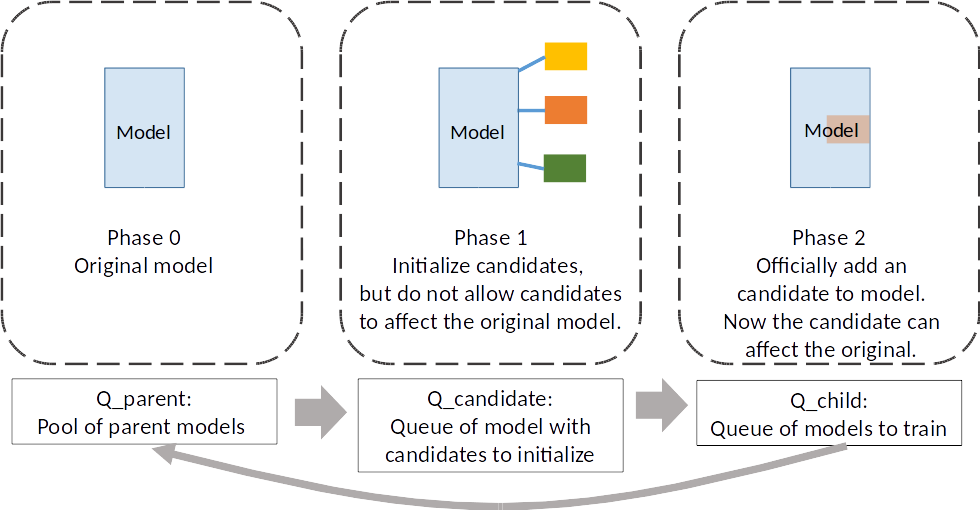
\includegraphics[width=0.8\textwidth,keepaspectratio]{\NASDIR/img/three_queues.png}
%    \caption{The search process repeat three steps: (a) choose a parent model, (b) initialize, train and select a number of candidate layers to add to the parent, and (c) finalize the selected candidates into the parent model and train for a few epochs.}
%    \label{fig:search_procedure}
%\end{figure*}


We propose a method to grow networks iteratively from existing models for searching cost-effective models. 
The network growth alternates between two phases. First, an existing parent model is expanded with candidate operations, and we train these operations along with the parent model to initialize them (Sec.~\ref{sec:candidate_init_and_select}). Second, based on feature selection techniques, we select from among the candidate operations, a small subset to permanently add to the parent model, and then finalize the model with some epochs of training starting from the initialization (Sec.~\ref{sec:candidate_finalize}). As we seek the most cost-effective models, we take a greedy approach to expand only the most cost-effective ones as parents (Sec.~\ref{sec:parent_choice}). 
The procedure is parallelized via a pool of GPU workers that perform training via backpropagation for both phases of growth. 

One reason for early NAS works~\citep{nas,NASCell,Real2018RegularizedEF} to have long search time is that candidate models are treated as independent and are trained separately. Recent works~\citep{Pham2018EfficientNA, Liu2018DARTSDA} exploit the similarity of candidate models by jointly training multiple models in a single joint super-graph of models in order to find the best sub-graph. However, designing such super-graph requires expert knowledge that may not exist for general data-sets. Furthermore, it is not clear how super-graph approaches can utilize existing trained models, an idea that has been shown in~\citep{Elsken2018EfficientMN} to also improve the search speed greatly and is important in production environments with large continuously streaming-in data. One contribution of this work is to expand existing models with small super-graphs of candidate operations, and select few of them to form a cost-efficient improvement of the original model. 

%I think we gain generality as no super-graph is needed, models can be warm started which DARTS and ENAS cannot do. We lose in terms of search time.

\begin{algorithm}[t]
\begin{algorithmic}[1]
\STATE \textbf{Input}: 
(1) $L_x$, the list of layers in the parent model (macro-search) or cell (cell-search) in topological order;
(2) $\text{is\_out}(x)$, whether layer $x$ can be $x_{out}$;
(3) frozen, whether to freeze the influence from candidates to the parent;
(4) $\lambda$, hyper parameter for feature selection.
\STATE $L'_x \leftarrow L_x$
\STATE $L_c \leftarrow \text{empty list}$
\FOR{$k$, $x_{out}$ in enumerate($L_x$)}
    \IF { not \text{is\_out}($x_{out}$)}
        \STATE continue
    \ENDIF
    \STATE $S$ $\leftarrow$ $L_x[:k]$ the sublist that ends before $x_{out}$.
    \STATE Uniformly randomly sample $I$ samples from $S$ without replacement as $x_{in,1}, ..., x_{in,I}$.

    %\STATE Initialize $\alpha_{i,j}$ randomly from Gaussian. 
    %\STATE Initialize parameters in $op_j(x_{in,i})$. 
    \IF { frozen }
        \STATE $x_c \leftarrow \sum _{i=1}^I \sum _{j=1}^J  \alpha^k_{i,j}op_j(\stopgradient (x_{in,i}))$.
    \ELSE
        \STATE $x_c \leftarrow \sum _{i=1}^I \sum _{j=1}^J  \alpha^k_{i,j}op_j(x_{in,i})$.
    \ENDIF
\STATE Insert the layer $x_c$ right before $x_{out}$ in $L'_x$.
\STATE Add $\lambda \sum _{i=1}^I \sum _{j=1}^J |\alpha^k_{i,j}|$ to the total loss of the model respented by $L'_x$.
\STATE Append $x_c$ to $L_c$.
\IF { frozen }
    \STATE Modify $x_{out}$ in $L'_x$ so that $x_{out} \leftarrow x_{out} + \stopforward (x_c)$.
\ELSE
    \STATE Modify $x_{out}$ in $L'_x$ so that $x_{out} \leftarrow x_{out} + x_c$.
\ENDIF
\ENDFOR
\STATE \textbf{Output}: (1) $L'_x$, the modified $L_x$ with candidates; 
(2) $L_c$, the list of $x_c$ created.
\end{algorithmic}
\caption{Initialize Candidates}
\label{alg:candidate_init}
\end{algorithm}

\begin{algorithm}[t]
\begin{algorithmic}[1]
\STATE \textbf{Inputs}: (1) $L'_x$, the list of layers of the model in topological order;
(2) $L_c$, list of selection modules in $L'_x$;
(3) $\alpha^k_{i,j}$, the learned weights candidate operations. 
\FOR{$x_c$ in $L_c$}
    \STATE Let $A = \{\alpha^{k}_{i,j}: i = 1,..., I, j = 1,..., J\}$  be the weights of operations in $x_c$.
    \STATE Sort $\{ |a| : a \in A \}$, and let the operations associated with the largest three value be $op_1, op_2, op_3$.
    \STATE Replace $x_k$ with $\text{proj}(\text{concat}(op_1, op_2, op_3))$ in $L'_x$.
\ENDFOR
\STATE Replace all $\stopforward (\cdot)$ and $\stopgradient (\cdot)$ with identity in $L'_x$.
\STATE \textbf{Output}: A modified $L'_x$ with selected operations.
\end{algorithmic}
\caption{Select and Finalize Candidates}
\label{alg:candidate_select}
\end{algorithm}

\subsection{Initialization of Candidates}
\label{sec:candidate_init_and_select}

\begin{figure}[t]
\centering
    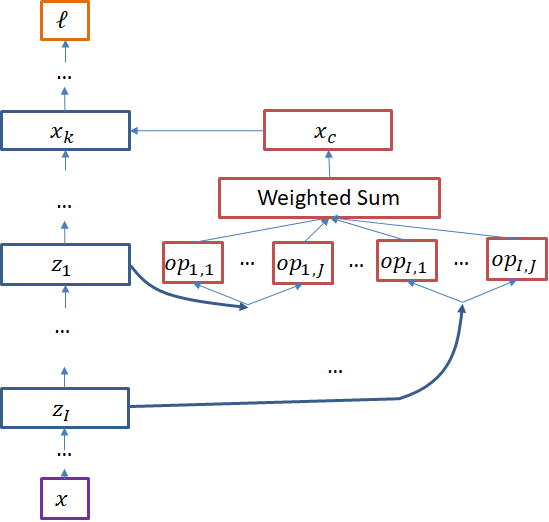
\includegraphics[width=0.4\textwidth, keepaspectratio]{\NASDIR/img/x_c_select.png}
    \caption{A selection module  where the parent model and the candidate operations are jointly trained (\petridishsoft).}
    \label{fig:x_c_select}
\end{figure}

Algorithm~\ref{alg:candidate_init} describes the procedure for expanding an existing model with feature selection modules to initialize and evaluate operations for forming shortcuts. Fig.~\ref{fig:x_c_select} illustrates a single selection module to add at layer $x_{out}$ of the parent model. 

\textbf{Output Layers.} The locations of $x_{out}$ are fixed through the search. In our cell-search, $x_{out}$ is the output of the cell. To fairly compare macro-search and cell-search, we start macro-search with the same network that cell-search does, and set $x_{out}$ to be the outputs of the cells in the initial network of the search. We detail the initial model later. 

\textbf{Input Layers.} The number of input layers $I$ of feature selection modules is set to be the number of layers in the parent model divided by the number of feature selection modules and then rounded up to the nearest integer. If $I$ is less than $2$, we set $I=2$. The input layers are then sampled uniformly at random without replacement from eligible layers. In cell-search, the eligible layers are those in the current cell or are inputs of the current cell. In macro-search, any layer topologically earlier than $x_{out}$ is eligible. 

\textbf{Operations.} 
To select a cost-effective set of operations for a shortcut from the inputs to the output, we initialize all possible $J$ operations on the inputs and combine them in a weighted sum to form the candidate layer $x_c$ as
\begin{align}
    x_c = \sum _{i=1}^I \sum_{j=1}^J \alpha_{i,j} op_j(x_{in,i}),
    \label{eq:x_c_select}
\end{align}
where we adapt the shorthand $op_{i,j} = op_j(x_{in,i})$ in the Fig.~\ref{fig:x_c_select}. 
The selection module then adds an additional loss to the total training loss:
\begin{align}
    \lambda \Vert \vec{\alpha} \Vert_1 = \sum_{i=1}^I \sum _{j=1}^J | \alpha _{i,j} |,
    \label{eq:x_c_select_loss}
\end{align} 
where $\lambda$ is a hyperparameter shared by all selection modules, and $\vec{\alpha}$ is the vector form of the scalar weights of the operations. This loss is inspired by the feature selection technique using L1 regularization~\citep{lasso}, known as Lasso, and similar approach has been successfully applied to model compression in neural networks~\citep{huang2017condensenet}. With the additional losses, backpropagation on the modified parent model simultaneously updates the parameters of the candidate operations and selects a subset of operations, because the operations with high absolute value of $\alpha$ are typically the more relevant features for $x_c$. 

\begin{figure}[t]
\centering
    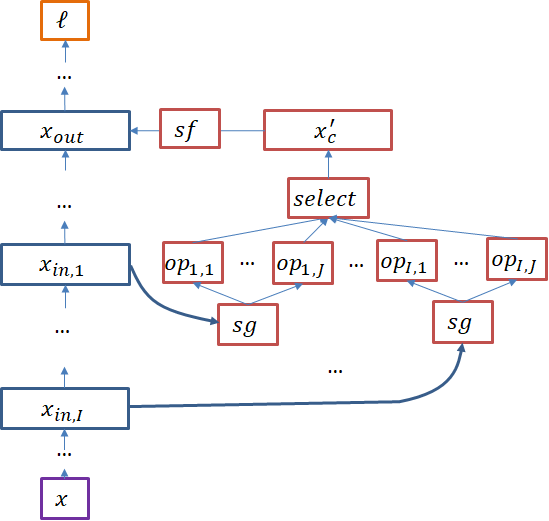
\includegraphics[width=0.4\textwidth, keepaspectratio]{\NASDIR/img/x_c_select_sf_sg.png}
    \caption{A selection module with stop-gradient and stop-forward to partially unfreeze the parent model (\petridishhard).}
    \label{fig:x_c_select_sf_sg}
\end{figure}

\textbf{Task Specific Details.}
For visual recognition tasks on CIFAR~\citep{cifar}, there are $J=6$ possible operations: 3x3, 5x5 and 7x7 depth-wise separable convolution, 3x3 max and average pooling, and identity. Following~\citep{NASCell,Real2018RegularizedEF,Pham2018EfficientNA}, separable convolutions are applied twice. 

The initial model for both macro and cell-search is a modified ResNet~\citep{resnet}, where we replace each 3x3 convolution with a 3x3 separable convolution. This is one of the simplest cell within the search space of existing literature~\citep{NASCell,Pham2018EfficientNA,Liu2018DARTSDA}.  Following ~\citep{nas,NASCell}, we have six regular cells for each of the three resolutions of feature maps.
A transition cell is in between each neighboring resolutions, and it also starts as a modified residual unit. Feature map channel sizes are doubled at transition cells, and the initial channel size is $F=32$, so that the found models of the proposed methods can be directly compared against the published results of~\citep{NASCell}. 

When we transfer the model to larger data-sets that require more than three resolutions, we use transition cells to first down-sample the image height and width to be no greater than 32 and then apply the found model. In macro-search, where no transition cells are specifically learned, we again use the the modified ResNet cells for initial transition in the transferred model.

\subsection{\petridishhard versus \petridishsoft Training.}
\label{sec:soft_vs_hard}
An interesting consideration is whether to freeze parameters of the parent models when we train and select the candidate layers. On one hand, most of our parent models are partially trained (more detail in Sec.~\ref{sec:candidate_finalize}) and the parent model contributes to the majority of the total computation, so we consider it very wasteful to freeze the parent parameters. On the other hand, if the parent model is frozen, different selection modules become independent of each other and may be easier to learn. Furthermore, freezing parent models prevents the newly initialized candidate layers from negatively affecting the parent model. C2~\citep{cascadecorr} thus adopts freezing the parent. 

Instead of strictly freezing or not freezing the parent model, we consider a tradeoff as illustrated in Fig.~\ref{fig:x_c_select_sf_sg}: we stop the influence of the selection module on the parent model during the selection phase, but we allow both parent model and the selection module to be learned at the same time. To do so, we leverage two operations ``stop-gradient''($\stopgradient$) to the inputs $x_{in,i}$ and ``stop-forward''($\stopforward$) to the final output $x_c$. The function $\stopgradient$ is identity during forward, i.e., $\stopgradient (x) = x$, but has a zero gradient during backpropagation, i.e., $\nabla \stopgradient(x) = 0$. The function $\stopforward$ is the opposite and is defined as $\stopforward (x) = x - \stopgradient (x)$, so it is zero during forward and $\nabla \stopforward (x) = \nabla x$ during backward pass.  
Hence, the final output to be added to the target location $x_{out}$ now becomes 
\begin{align}
    \stopforward (x'_c) =  \stopforward \big(\sum _{i=1}^I \sum_{j=1}^J \alpha_{i,j} op_j( \stopgradient( x_{in,i} ) ) \big). 
    \label{eq:x_c_select_sf_sg}
\end{align}
As this term is zero during forward computation, the parent model's prediction is unaffected. This term also has a zero gradient with respect to all the input $x_{in,i}$ thanks to $\stopgradient$. This blocks the influence from the candidate layers to the parent model, analogous to how C2~\citep{cascadecorr} freezes learned neurons while initializing new neurons. 

One can also understand Eq.~\ref{eq:x_c_select_sf_sg} by considering the linear loss
\begin{align}
   \langle \nabla_{x_{out}} \ell, x'_c \rangle =  
   \langle \nabla_{x_{out}} \ell, \sum _{i=1}^I \sum_{j=1}^J \alpha_{i,j} op_j( \stopgradient( x_{in,i} ) ) \rangle,
    \label{eq:x_c_linear_loss}
\end{align}
where $\nabla_{x_{out}} \ell$ is the gradient of the prediction loss with respect to the tensor $x_{out}$. We note that the gradient of the prediction loss with respect to parameters in $x'_c$ is the same as gradients of Eq.~\ref{eq:x_c_linear_loss} with respect to the same parameters. Hence, the construction of $x'_c$ is in fact encouraging the selection module to fit its output $x'_c$ to match the negative gradient $-\nabla_{x_{out}} \ell$ of the prediction loss.


In our experiments (Sec.~\ref{sec:experiment_soft_vs_hard}), we compare the above version of candidate training (\petridishhard) against the version where the parent parameters are not frozen during candidate training (\petridishsoft). 




\subsection{Candidate Finalization}
\label{sec:candidate_finalize}

\begin{figure}[t]
\centering
    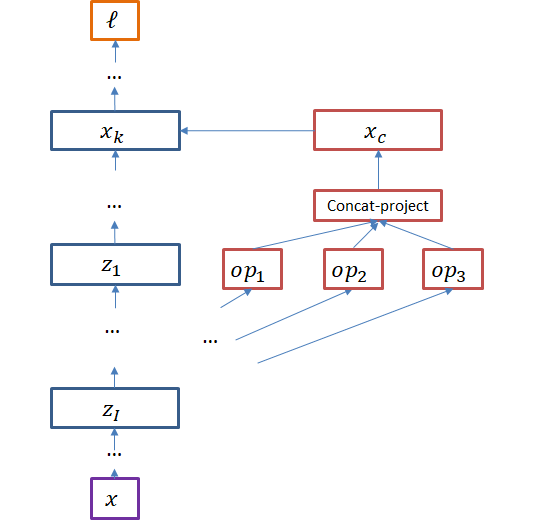
\includegraphics[width=0.4\textwidth, keepaspectratio]{\NASDIR/img/x_c_select_final.png}
    \caption{Weighted sum is replaced with concat-projection, when the top operations are chosen. Any $\stopforward$ or $\stopgradient$ are also removed.}
    \label{fig:x_c_select_final}
\end{figure}

Algorithm~\ref{alg:candidate_select} describes how we select and finalize the initialized models. 
The absolute value of the weights $\alpha_{i,j}$ convey the importance of the associated candidate operations. Upon finishing training the candidate layers with a few epochs, we keep the top three operations for each selection module in terms of the corresponding $| \alpha _{i,j} |$. 
Other operations are removed. In our experiments in Sec.~\ref{sec:sum_vs_cat_proj}, we found a simple modification to be crucial for the final model cost-efficiency: instead of combining the selected operations in a weighted sum as in the selection phase, we concatenate the feature maps along the feature dimension, and project the result with 1x1 convolution to the same channel size as the target $x_{out}$ before summing them together to replace $x_{out}$, as illustrated in Fig.~\ref{fig:x_c_select_final}. This modification is in fact implicitly used by most of the existing neural architecture search works~\citep{NASCell,Pham2018EfficientNA}, where the layers within a cell is concatenated to form the cell output, and any operations on the output first project it to the same channel size as layers that are not cell outputs. We train the finalized model for a few epochs starting with the parameters from the selection phase. 





\subsection{Parent Selection}
\label{sec:parent_choice}


%\begin{algorithm}[t]
%\begin{algorithmic}[1]
%\STATE Set $T = $
%\STATE \textbf{Input}: (1) a pool of trained models, $Q_{p}$; 
%(2) search tree depth for each model $m$, $d(m)$, e.g., the initial model has $d(m) = 0$; 
%(3) number of times each model $m$ is chosen as parents, $n(m)$. 
%\STATE Compute the lower convex hull of the models on the plot of test-time computational costs versus error rates of models. 
%\STATE Sample a model $m$ on the hull, with probability defined by Eq.~\ref{eq:parent_weight}. 
%\STATE \textbf{Output}:  A model $m$ selected as the parent model. 
%\end{algorithmic}
%\caption{Select Parent( )}
%\label{alg:select_parent}
%\end{algorithm}


The goal of architecture search is to efficiently find small yet accurate
neural networks. In this work, we take a greedy approach which aims to build low cost accurate models. A model is considered the most
cost-effective, if there do not exist other models that are both less
costly and test time and more accurate. Such models exactly lie on the
Pareto-frontier of the scatter plot of test-time computation (in
FLOPS) versus error rate. We also note that given two models on the
scatter plot, any average performance on the line segment between them
can be achieved by mixing the use of the two models with appropriate
probabilities. Hence, we further restrict the most cost-effective
models to be on the lower convex hull of the cost versus error plot.

We initialize the parent pool with a single simple data-set-dependent 
model, which we detail in the experiments, and the pool expands during 
the search.
As a result, we need to balance the exploration and exploitation of the 
parent models. 
In this work, given a model $m$ on the lower convex hull, we weigh its 
probability to become a parent model based on two values.
First, the probability should decrease with the number of times the model 
is chosen before, $n(m)$. Second, as we expand the models from an initial
model, all models are naturally on a search tree rooted at the initial model.
We call the depth of $m$ on the search tree $d(m)$, e.g., 
the initial model has depth 0; its children with candidate selection
models have depth 1; the grandchildren with finalized candidates have depth 2. 
The probability
should increase with $d(m)$, because the number of possible models grow at 
least exponentially with the search tree depth. Combining these two insights, 
we weight the probability of choosing a hull point to be:
\begin{align}
    Pr(\text{$m$ is chosen}) \propto exp( (d(m) - d_{max}) n(m) ),
    \label{eq:parent_weight}
\end{align}
where $d_{max}$ is the maximum allowed search depth. We set 
$d_{max} = 16$ to prevent searching overly complex models. 

A finalized and trained model from Sec.~\ref{sec:candidate_finalize} is evaluated on a validation set, and is added to the parent pool if it is on the lower convex hull of the plot of test-time computation versus validation error rates. We also remove from the parent pool the models that are no longer on the lower convex hull, when the hull is changed by new models. 
    
\section{Experiment}
\label{sec:nas_experiment}

%%%%%%%%%%%%%%%%%%%%%%%% 
% Experimental questions
%%%%%%%%%%%%%%%%%%%%%%%%
%\subsection{Experimental questions}
%\begin{enumerate}
%\item 
%\end{enumerate}


%%%%%%%%%%%%%%%%%%%%%%%% 
% Data-sets
%%%%%%%%%%%%%%%%%%%%%%%%

%%%%%%%%%%%%%%%%%%%%%%%% 
% Eval metric
%%%%%%%%%%%%%%%%%%%%%%%%
%\subsection{Evaluation Metrics}

%\begin{enumerate}
%    \item For fixed search space and training parameters, we can 
%    compare the best found model validation error after the same number of 
%    models are trained.
    %\item For a more general comparison among search algorithms, we plot the curves of the best validation error versus FLOPs spent on training. Then the lower curves represent algorithms that find the most accurate models faster.
    %\item While the previous two metrics focus on how fast the search can find the most accurate models, they do not consider the cost-efficiency of the searched models. To evaluate the cost-efficiency, we represent the cost-efficiency of searched models by the lower convex hull of validation error versus model computational cost, measured in FLOPs. The more close the hull is to the origin, the more cost efficient the found models are. We can compare algorithms by comparing their performance convex hulls. 
%\end{enumerate}


%%%%%%%%%%%%%%%%%%%%%%%% 
% Parent choice Experiment
%%%%%%%%%%%%%%%%%%%%%%%%


%%%%%%%%%%%%%%%%%%%%%%%% 
% Visual Recognition Data-sets
%%%%%%%%%%%%%%%%%%%%%%%%
\subsection{Search Results on CIFAR10}
\label{sec:experiment_cifar10_search}

\textbf{Set-up.}
We first apply the proposed algorithm to search for architectures on CIFAR-10~\citep{cifar}. During search, we use a fixed set of 45000 training images for training, and 5000 for validation. Both candidate initialization and finalization are trained for 80 epochs, with a batch size 32 and a learning rate that decays from 0.025 to 0 in cosine decay~\citep{cosine_lr}. We apply drop-out~\citep{larsson2016fractalnet} and cut-out~\citep{cutout} during search. The final found model is trained from scratch using the same parameters, except that it trains on all 50000 training images, and spends 600 epochs. 


\textbf{Search Results.} 
Table~\ref{tab:cifar10_search} depicts the test-errors, model parameters, and search computation of the proposed methods along with many state-of-the-art methods.
\Petridish cell search finds a model with 2.79\% error rate with 2.8M parameters, in 15.3 GPU-days. This performance is similar to or better than cell search methods. \Petridish macro search finds a model that achieves 2.86\% error rate using 4.8M parameters in 27.2 GPU-days . This is significantly better than any previous macro search results, 
and showcases that macro search can find cost-effective architectures that are previously only found through cell search. 

\textbf{Importance of initial models.}
Table~\ref{tab:cifar10_search} also showcase the impact of initial models to the final results of architecture search. This is an important topic, because existing literature has been moving away from macro architecture search, as early works~\citep{NASCell,Pham2018EfficientNA,Real2018RegularizedEF} have shown cell search results tend to be superior than those from macro search. However, this result may be explained away by the superior initial models of cell search: the initial model of \Petridish is one of the simplest model that any of the listed cell search methods would propose and evaluate, and it already achieves 4.6\% error rate using only 0.4M parameters, a result that is on-par or better than many macro search results. 


\begin{table*}[t]
    \centering
    \caption{Comparison against state-of-the-art recognition results on CIFAR-10. Results marked with $\dagger$ are not trained with cutout. The first block represents approaches for macro-search. The second block represents approaches for cell-search. 
    }
    \begin{tabular}{l|cccc}
    \hline
\multirow{ 2}{*}{\textbf{Method} }
        &  \textbf{\# params} 
        &  \textbf{Search } 
        &  \textbf{Test Error } \\
        &  (mil.)
        &  (GPU-Days)
        &  (\%)\\
\hline
\citet{nas}$^{\dagger}$
    &  7.1 &  1680+ &  4.47  \\
\citet{nas} + more filters$^{\dagger}$
    &  37.4 &   1680+ &  3.65   \\
\citet{Real2017EvoNet}$^{\dagger}$
    &  5.4 &   2500 &  5.4  \\
ENAS macro~\citep{Pham2018EfficientNA}$^{\dagger}$
    &  21.3 &  0.32 &  4.23 \\
ENAS macro + more filters$^{\dagger}$
    &  38 &   0.32 &  3.87 \\
Lemonade I~\citep{Elsken2018EfficientMN}
    &  8.9 &    56 &  3.37 \\
\hline
\Petridish initial model ($N=6$, $F=32$)
    & 0.4 &  -- & 4.6 \\
%\Petridish macro without DropPath
%    & 3.1 & 6 & 3.38 \\
\textbf{\Petridish macro} 
    & \textbf{4.8} & 27.2 & \textbf{2.86} \\
%\Petridish macro (start at $N$=3, $F$=32)
%    & 2.7 & 18 & 3.44 \\
\hline \hline
NasNet-A~\citep{NASCell}
    &  3.3 &    1800 &  2.65   \\
AmoebaNet-A~\citep{Real2018RegularizedEF}
    &  3.2 &  3150 &  3.3  \\
AmoebaNet-B~\citep{Real2018RegularizedEF} 
    &  2.8 &   3150 &  2.55 \\ 
PNAS~\citep{Liu2017ProgressiveNA}$^{\dagger}$
    &  3.2 &  225 &  3.41 \\
Heirarchical NAS~\citep{Liu2018HierNA}$^{\dagger}$
    &  15.7 &    300 &  3.75 \\ 
ENAS cell~\citep{Pham2018EfficientNA}
    &  4.6 &  0.45 &  2.89 \\ 
ENAS cell~\citep{Pham2018EfficientNA}$^{\dagger}$
    &  4.6 &  0.45 &  3.54 \\ 
Lemonade II~\citep{Elsken2018EfficientMN}
    &  3.98 &  56 &  3.50 \\
Darts~\citep{Liu2018DARTSDA}
    &  3.4 &   4 &  2.83 \\ 
Darts random~\citep{Liu2018DARTSDA}
    & 3.1 & -- & 3.49 \\
\citet{CaiPathLevel} 
    & 5.7 &  8  & 2.49 \\
\citet{NAONet}$^{\dagger}$
    & 3.3 & 0.4 & 3.53 \\
\hline
\textbf{\Petridish cell}
    & \textbf{2.8} & 15.3 & \textbf{2.79} \\
%\Petridish cell + more filters
%    & 3.5 & 6 & 3.05 \\
\hline
    \end{tabular}
    \label{tab:cifar10_search}
\end{table*}



\subsection{Transfer to CIFAR100 and ImageNet}
\label{sec:experiment_vision_transfer}



\begin{table*}[t]
    \centering
    \caption{ILSVRC2012 transfer results. \Petridish uses \petridishhard and the concat-projection (CP) modification by default. The last six rows of the tables are for ablation studies.
    }
    \begin{tabular}{l|cccc}
    \hline
\multirow{ 2}{*}{\textbf{Method} }
        &  \textbf{\# params} 
        &  \textbf{\# multi-add}
        &  \textbf{Search}
        &  \textbf{top-1 Test Error } \\
        &  (mil.)
        &  (mil.)
        &  (GPU-Days)
        &  (\%)\\
\hline
Inception-v1 (Szegedy et al., 2015)
    & 6.6 & 1448 & -- & 30.2 \\
MobileNetV2 (Sandler et al., 2018)
    & 6.9 & 585 & -- & 28.0 \\
\hline
NASNet-A (Zoph et al., 2017) 
    & 5.3 & 564 & 1800 & 26.0 \\
NASNet-B (Zoph et al., 2017) 
    & 5.3 & 488 & 1800 & 27.2 \\
AmoebaNet-A (Real et al., 2018)
    & 5.1 & 555 & 3150 & 25.5 \\
PNAS (Liu et al., 2017a)
    & 5.1 & 588 & 225  & 25.8 \\
DARTS (Liu et al., 2018)
    & 4.9 & 595 & 4    & 26.9 \\
\hline
\textbf{\Petridish macro} (F=32) %828
    & 4.9 & 593 & 27.2 & 29.4 \\
\textbf{\Petridish macro} (F=48) %822
    & 10.4 & 1247 & 27.2 & 25.2 \\
\hline
\textbf{\Petridish cell} (F=40) %841
    & 4.4 & 583 & 15.3 &  26.9 \\
\textbf{\Petridish cell} (F=48) %824
    & 6.2 & 813 & 15.3 & 25.4 \\
\hline
\hline
\Petridish \petridishsoft macro (F=48) %839
    & 4.6 & 587 & 22.7 & 29.0 \\
\Petridish \petridishsoft cell (F=32) %843,842,833,834
    & 4.0 & 546 & 20.6 & 32.8 \\
\hline
\hline
\PetridishWS macro(F=48) %808
    & 5.9 & 756 & 29.5 & 32.5\\
\PetridishCP macro (F=36) %845
    & 5.4 & 680 & 29.5 & 29.1 \\
\PetridishWS cell (F=48) %810
    & 3.3 & 477 & 22.8 & 32.7\\
\PetridishCP cell  (F=44) %848
    & 4.7 & 630 & 22.8 & 27.2 \\
\hline  \end{tabular}
    \label{tab:imagenet_compare}
\end{table*}



For ILSVRC2012~\citep{ILSVRC15}, we take the standard data augmentation approach of~\citep{resnet}, and use 224x224 input images. To utilize the found architecture that are designed for 32x32 images, we apply a 3x3 conv with stride 2 to transform the RGB-color into $F / 4$ channels, and then apply two transition cells (as stated in Sec.~\ref{sec:candidate_init_and_select}) to down-sample the feature map to 28x28 and $F$ channels. We treat the resulting tensor as the input image for the found architectures. 

The top-1 error rate, the number of model parameters and the test-time computational cost in terms of mult-adds are shown in Table~\ref{tab:imagenet_compare}. Model of \Petridish cell-search achieves 26.9\% error rate using 4.4M parameters and 587M multi-adds, which is on par with state-of-the-art results listed in the second block of Table~\ref{tab:imagenet_compare}. By utilizing feature selection techniques to evaluating multiple model expansions at the same time, \Petridish is able to find models faster by one or two orders of magnitudes than early methods that train models independently, such as NASNet~\citep{NASCell}, AmoebaNet~\citep{Real2018RegularizedEF}, and PNAS~\citep{Liu2017ProgressiveNA}.  
In comparison to super-graph methods such as DARTS~\citep{Liu2018DARTSDA}, \Petridish cell-search sacrifices about four times search speed for the flexibility to grow from existing models. 

We also observe that the model from \Petridish macro-search achieves 29.4\% error rate using 4.9M parameters and 593M multi-adds, a comparable result to the human-designed models in the first block of Table~\ref{tab:imagenet_compare}. To the best of our knowledge, this is one of the first successful result to transfer macro-search results on CIFAR to ImageNet, showing that macro-search results can be transferred. 
However, we do observe the gap in error rates between \Petridish macro from \Petridish cell, suggesting that giving full freedom of choosing input layers as in \Petridish macro may reduce the search speed to find a state-of-the-art model.


\subsection{Weighted Sum versus Concatenation-Projection}
\label{sec:sum_vs_cat_proj}

After selecting the operations in Sec.~\ref{sec:candidate_finalize}, we concatenate them and project the result with 1x1 conv so that the result can be added to the output layer $x_{out}$. 
Here we empirically justify this design choice.

We first consider applying the switch only to the final reported model, i.e., we do not use CP during search, and only switch all feature selection weighted sums (WS) to CP in the final model, which we train from scratch to report results. We call this variant as \PetridishCP, and the variant where we never switching to CP as \PetridishWS. Since CP incurs additional computation to the model, we increase the channel size of \PetridishWS so that the two variants have similar test-time multi-adds for fair comparisons. 
The last four rows of Table~\ref{tab:imagenet_compare} showcases this comparison on the transfer results on ImageNet, and \PetridishCP achieves lower errors than \PetridishWS while using similar amounts parameters and multi-adds. This suggests that the proposed switch to CP from WS is a more cost-effective way to improve model predictive power than increasing model channel sizes when it is applied to the found models.

We next consider switching to CP during search, which \Petridish does by default in Alg.~\ref{alg:candidate_select}, and evaluate its impact of the switch, because it is unclear that the additional computation of CP is out-weighed by the predictive power of the improved models. Comparing \PetridishCP against \Petridish in Table~\ref{tab:imagenet_compare}, we observe that for both cell and macro searches, models of \Petridish are both more accurate and less expensive in test-time computation and it takes similar or shorter time for \Petridish to find the models than \PetridishCP did. 




\subsection{\petridishhard versus \petridishsoft}
\label{sec:experiment_soft_vs_hard}

In Sec.~\ref{sec:soft_vs_hard}, we apply $\stopforward$ and $\stopgradient$ to block the influence of feature selection modules to the parent models, which we called \petridishhard. This section empirically studies this design choice versus the variant \petridishsoft, where $\stopforward$ and $\stopgradient$ are simply replaced with identity. Table~\ref{tab:imagenet_compare} showcases the transfer results of \petridishhard (\Petridish) and \petridishsoft to ImageNet. We first compare \Petridish cell (F=40) with \petridishsoft cell (F=32), two models that have similar computational cost but very different accuracy, and we observe that \petridishhard leads to a better model than \petridishsoft for cell-search. In macro-search, the comparison between \petridishhard and \petridishsoft appears to be non-conclusive (\Petridish macro (F=32) versus \petridishsoft macro (F=48)), as both methods find models of similar complexity and accuracy using similar search time. 


\section{Conclusion and Discussion}
\label{sec:conclusion}
In this work, 

%
%\bibliographystyle{sty_bst/icml.bst}
%\bibliography{network_search}
%
%\appendix
\section{Sampling Parents on the Lower Convex Hull}

\subsection{Intuitions}
\label{sec:candidate_parent_intuition}

To choose models on the convex hull in a fair manner, we have the following intuitions.
\begin{enumerate}
\item 
Since we want to maximize the improvement of the pareto front per unit cost spent during training, we should discount the probability of a model to be chosen, $p(m)$, by the cost of the model $c(m)$, which is proportional to the training cost.
\begin{align}
    p(m) \propto \frac{1}{c(m)}
\end{align}

\item 
In Sec.~\ref{sec:candidate_init_and_select}, we choose a number of input layers for each selection modules. The number of possible inputs is $d(m) + 2$, the editing distance from the current model $m$ to the seed model. Among them, we choose $\eta d(m)$ as input layers, where $\eta$ is a constant in $(0,1]$ deciding the growth rate of the model. 
Hence, each cell in model $m$ has ${ d(m) + 2 \choose \eta d(m) }$ possible selection modules to be attached with. 

In cell search, there are two free cells, normal and reduction cells. In macro search, every cell is free, and in the case of visual recognition, there are 20 cells. Let $f(m)$ be the number of free cells in the model $m$. Then we should sample a model with a number of times that is proportional to its possible selection modules, in order to uniformly sample all models uniformly at random. Hence, we have

\begin{align}
    p(m) \propto { d(m) + 2 \choose \eta d(m) } ^{f(m)}.
\end{align}



\item 
When we have chosen a model $m$ for $n(m)$ times, we should sample it with probability discounted by a factor $\frac{1}{n(m) + 1}$, because assuming uniformly sampling possible children models, the next one is the best with a probability $\frac{1}{n(m) + 1}$
\begin{align}
    p(m) \propto \frac{1}{n(m) + 1}
\end{align}

\item 
\citet{Elsken2018EfficientMN} use inverse of probability density to sample the models, where the density function is based on the model parameter sizes. This also supports the intuition that 
when models are clustered together, i.e., having similar computational cost, and/or accuracy, we should discount their probability, because they only represent a small portion of the convex hull. 
To compute the probability density at the computational cost of model $m$, we use non-parameter regression with the points on the convex hull. E.g., we can use Gaussian kernel with the median distance as the kernel width to estimate the density as $pdf(c(m))$. Then we weight the probability of choosing $m$ as the parent with 
\begin{align}
    p(m) \propto \frac{1}{pdf(c(m))}
\end{align}

\item

As models grow larger and and more accurate, we expect to have smaller fraction of candidate expansion to be able to positively affect the accuracy and/or cost-effectiveness of the model. Hence, we may want to sample the larger and/or more accurate models more often than the early and inaccurate models, in order to achieve uniform improvement of the convex hull. If the fraction of beneficial candidate expansions $b(m)$ is a constant, then item (2) above already addresses this problem. If the fraction is indeed decreasing, then we need to set $p(m)$  inversely proportional to this fraction, i.e.,
\begin{align}
    p(m) \propto \frac{1}{b(m)}.
\end{align} 
However, this is difficult to achieve, because $b(m)$ cannot be estimated and $b(m)$ can be zero. 

A workaround to estimate $b(m)$ is with the proportion of children of the parent of $m$ that we have sampled before finding $m$, $\tilde{b}(m)$. This is also a work around for the problem of $b(m) = 0$, because by finding $m$, the parent of $m$ definitely has non-zero $b()$. 
Hence, we instead have 
\begin{align}
    p(m) \propto \frac{1}{\tilde{b}(m)}.
\end{align}

\end{enumerate}


\subsection{Possible Algorithms}

\subsubsection{Greedy Expansion}
The algorithm is as follows.
\begin{enumerate}
    \item Sort the models in the order of their error rates in increasing order as $m_1, m_2,...$
    \item While we have not chosen a model, we loop with $i =1,2,3,$ and so on. For each $i$, we choose $m_i$ with probability $p(m_i) = \frac{1}{n(m_i) + 1}$. 
\end{enumerate}

\subsubsection{Intuition Kitchen Sink}
Combining the intuitions of Sec.~\ref{sec:candidate_parent_intuition}, we have the probability to choose model $m$ to be 
\begin{align}
    p(m) \propto \frac{ {d(m) + 2 \choose \eta d(m) }^{f(m)} }{pdf(c(m)) c(m) (n(m) + 1) \tilde{b}(m)  }.
\end{align}


\section{Bi-level optimization}
\label{sec:nas_bi_level_optimization}


%\end{document}
